\documentclass[tikz]{standalone}
\usepackage{pgfplots}
\pgfplotsset{compat=1.15}
\usepackage{mathrsfs}
\usetikzlibrary{arrows,calc}
\usepackage{tkz-euclide}

\pagestyle{empty}

\definecolor{AngleClr}{rgb}{0,0.39215686274509803,0}
\definecolor{ShapeClr}{rgb}{0.6,0.2,0}
\definecolor{BlueClr}{RGB}{13,93,184}

\begin{document}

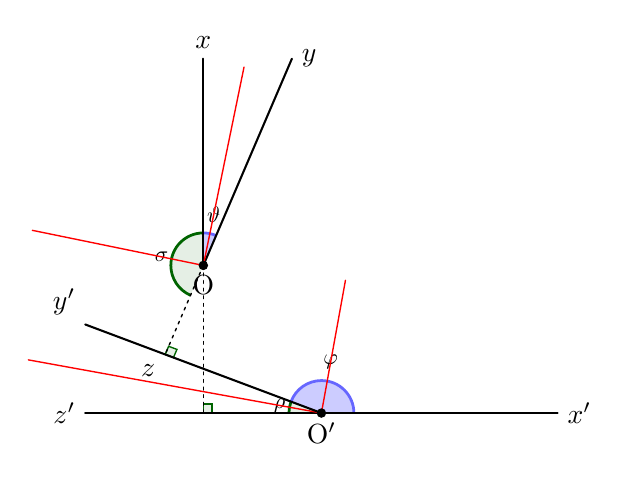
\begin{tikzpicture}[scale=.75]
\tkzSetUpLine[line width=1pt,color=black]
\tkzSetUpPoint[fill=black]

\tkzDefPoints{-4/1/z,-2/-1.5/z',0/1/O,2/-1.5/O',0/4.5/x,6/-1.5/x',1.5/4.5/y,-2/0/y'}

\tkzInterLL(y,O)(O',y') \tkzGetPoint{K}
\tkzInterLL(x,O)(O',z') \tkzGetPoint{K'}

\tkzDefLine[bisector](x,O,y)\tkzGetPoint{aa}
\tkzDefLine[bisector](x,O,K)\tkzGetPoint{bb}

\tkzDefPointOnLine[pos=1](O,aa) \tkzGetPoint{a}
\tkzDefPointOnLine[pos=4.2](O,bb) \tkzGetPoint{b}

\tkzDefLine[bisector](x',O',y')\tkzGetPoint{aa'}
\tkzDefLine[bisector](y',O',z')\tkzGetPoint{bb'}

\tkzDefPointOnLine[pos=3.2](O',aa') \tkzGetPoint{a'}
\tkzDefPointOnLine[pos=1.2](O',bb') \tkzGetPoint{b'}

\tkzFillAngles[fill=AngleClr,size=.55,fill opacity=0.1](x,O,K)
\tkzMarkAngles[line width=1pt,size=.55,color=AngleClr](x,O,K)
\tkzLabelAngles[scale=0.8,pos=0.9](x,O,K){$\sigma$}

\tkzFillAngles[fill=blue!20!white,size=.55](y,O,x)
\tkzMarkAngles[line width=1pt,size=.55,color=blue!60!white](y,O,x)
\tkzLabelAngles[scale=0.8,pos=1.1](y,O,x){$\vartheta$}

\tkzFillAngles[fill=blue!20!white,size=.55](x',O',y')
\tkzMarkAngles[line width=1pt,size=.55,color=blue!60!white](x',O',y')
\tkzLabelAngles[scale=0.8,pos=1.1](x',O',y'){$\varphi$}

\tkzFillAngles[fill=AngleClr,size=.55,fill opacity=0.1](y',O',z')
\tkzMarkAngles[line width=1pt,size=.55,color=AngleClr](y',O',z')
\tkzLabelAngles[scale=0.8,pos=0.9](y',O',z'){$\rho$}

% \tkzFillAngles[fill=blue!20!white,size=.55](x,K,y')
% \tkzMarkAngles[line width=1pt,size=.55,color=blue!60!white](x,K,y')
% \tkzLabelAngles[scale=0.8,pos=1.1](x,K,y'){$\omega$}

\tkzMarkRightAngles[line width=0.5pt, size=.15,color=AngleClr,fill=AngleClr,fill opacity=0.1](O,K,O' O,K',O')

\tkzDrawSegment[line width=0.75pt](O,x)
\tkzDrawSegments[line width=0.75pt](z',x' O,y)
\tkzDrawSegments[red,line width=0.5pt](O,a O,b)
\tkzDrawSegments[red,line width=0.5pt](O',a' O',b')
\tkzDrawSegment[line width=0.75pt](O',y')
\tkzDrawSegments[line width=0.5pt,color=black,dashed,dash pattern=on 1pt off 1.75pt](O,K O,K')

\tkzDrawPoints[size=3](O,O') % ,K)

\tkzLabelPoint[below](O){$\rm O$}
\tkzLabelPoint[below](O'){$\rm O'$}
% \tkzLabelPoint[below](K){$\rm K$}

\tkzLabelPoint[below left](K){$z$}
\tkzLabelPoint[left](z'){$z'$}
\tkzLabelPoint[above](x){$x$}
\tkzLabelPoint[right](x'){$x'$}

\tkzLabelPoint[right](y){$y$}
\tkzLabelPoint[above left](y'){$y'$}


\end{tikzpicture}

\end{document}
